\section{Methodology}
This chapter presents the conceptual framework underpinning the system's design philosophy, followed by a detailed account of the system architecture, hardware construction, feed hopper and trough volume calculations, feed and water dispensing mechanism, environmental and consumption sensing strategy, wired communication protocol, and system performance evaluation metrics.

\subsection{Conceptual Framework}

\begin{figure}[htbp]
  \centering
  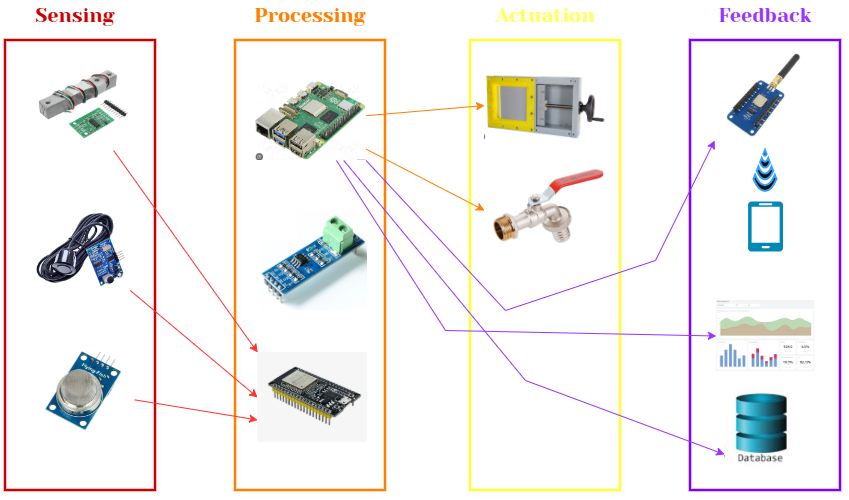
\includegraphics[width=0.8\columnwidth]{ConceptualFramework.png}
  \caption{Conceptual Framework}
  \label{fig:conceptual_framework}
\end{figure}

As illustrated in Figure \ref{fig:conceptual_framework}, the system is conceptualized as a closed-loop precision livestock management platform grounded in two theoretical underpinnings: Precision Agriculture Theory---which frames sensor-driven, individualized resource delivery as the basis for efficient swine production---and Feedback Control Systems Theory, which models each feeder module as a node whose output (feed and water dispensed) is continuously logged and compared against defined consumption baselines to flag deviations indicative of illness.

The system's operational logic spans four functional layers:
\begin{itemize}
  \item \textbf{Layer 1 -- Sensing (Input):} Each feeder module integrates a load cell with an HX711 24-bit ADC for gravimetric feed measurement, a waterproof ultrasonic sensor (e.g., JSN-SR04T) for water level monitoring, and an MQ-135 electrochemical sensor for ammonia air-quality monitoring.
  \item \textbf{Layer 2 -- Processing and Decision (Control):} Each feeder module's ESP32 microcontroller evaluates sensor readings against pre-established rolling-window consumption baselines. Deviations beyond a defined threshold are flagged as health alerts and relayed to the main control module via the RS-485 wired bus. The Raspberry Pi central controller processes incoming data, executes alert logic, and manages the touchscreen dashboard.
  \item \textbf{Layer 3 -- Actuation (Output):} Upon a scheduled or manually triggered feeding event, the main control module commands the solenoid-actuated sliding plate valve at the base of the truncated-pyramid hopper to open for a calibrated duration, dispensing a gravimetrically verified quantity of feed into each trough. Water is dispensed through a solenoid valve when the sensor detects the water level has dropped below a predefined threshold. This valve can also be manually overridden using an active-high push button on pin RA0 to ensure rapid caretaker intervention if needed.
  \item \textbf{Layer 4 -- Feedback, Logging, and Remote Notification:} All sensor readings, dispensing events, and alerts are timestamped and stored in a local SQLite database on the Raspberry Pi. In addition to displaying alerts on the local touchscreen dashboard, the system utilizes a LoRa (Long Range) transceiver to transmit critical health and environmental alerts to a remote LoRa-GSM gateway positioned outside the piggery. Upon receiving the LoRa payload, the gateway forwards the alert as an SMS message to the caretaker's mobile phone, ensuring real-time remote notification regardless of the caretaker's location on the farm.
\end{itemize}

\subsection{System Architecture: Distributed Software Workflow}

\begin{figure}[h]
  \centering
  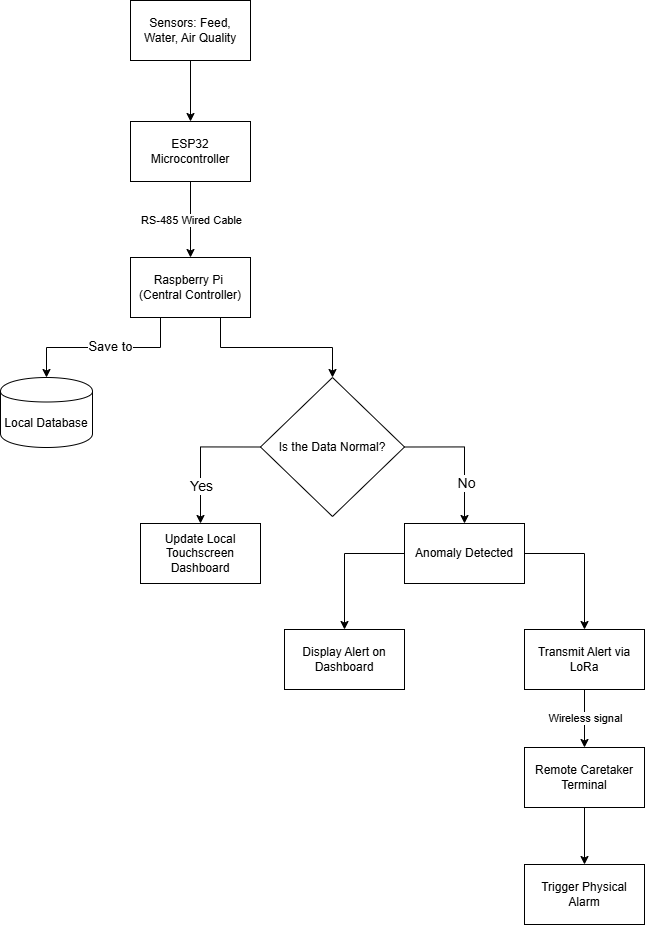
\includegraphics[width=0.8\columnwidth]{SoftwareDiagram.png}
  \caption{System Flowchart}
  \label{fig:software_flowchart}
\end{figure}

The system employs a distributed, hierarchical software architecture to decouple real-time hardware interfacing from high-level data orchestration. As illustrated in Figure \ref{fig:software_flowchart}, the software workflow operates in a continuous loop. Data acquisition begins at the edge nodes where the ESP32 samples the sensors via hardware interrupts. The Raspberry Pi systematically polls these nodes over the RS-485 bus. Upon receiving the telemetry, the Python backend writes the raw data to the SQLite database and passes it to the Analytical Engine. If the data falls within normal baseline parameters, it is pushed to the Flask frontend for live dashboard visualization. If an anomaly is detected, the system simultaneously triggers a visual alert on the local touchscreen dashboard and transmits an alert payload via LoRa to the remote LoRa-GSM gateway, which forwards it as an SMS to the caretaker's mobile phone.

\begin{itemize}
  \item \textbf{Edge Intelligence (Feeder Nodes):} Each node is governed by an ESP32 dual-core microcontroller. One core is dedicated to continuous sensor polling (load cell and flow meter) using hardware interrupts and the HX711 24-bit ADC, while the second core manages a MODBUS RTU slave stack. Telemetry is stored in a local register map, allowing the master to retrieve data asynchronously without blocking sensor acquisition.
  \item \textbf{Central Orchestration (Main Module):} A Raspberry Pi serves as the MODBUS RTU master, implementing a sequential polling loop via the RS-485 bus. The main module is co-located with the central hopper---a $0.18\text{ m}^3$-capacity truncated-pyramid storage unit---from which feed is gravity-fed through an auger conveyor to individual feeder nodes. The master logic is divided into four primary services:
    \begin{itemize}
      \item \textbf{Poller Service:} Executes MODBUS read commands at 1-second intervals to aggregate per-pen telemetry.
      \item \textbf{Analytical Engine:} Implements the rolling-window anomaly detection logic, comparing incoming data against the SQLite-persisted baseline.
      \item \textbf{Command Service:} Dispatches metered dispensing instructions based on the pre-configured feeding schedule or manual overrides.
      \item \textbf{LoRa Alert Service:} Interfaces with a connected LoRa transceiver module via SPI or UART. When the Analytical Engine flags an anomaly based on the rolling-window baseline, this service encodes the alert data into a lightweight payload and transmits it over the LoRa link to the remote LoRa-GSM gateway for SMS forwarding to the caretaker's mobile phone.
    \end{itemize}
  \item \textbf{Remote LoRa-GSM Gateway:} A secondary edge device positioned outside the piggery in a location with adequate cellular coverage. It receives incoming LoRa alert payloads and forwards them as SMS messages to the caretaker's registered mobile phone number via an onboard GSM module, enabling immediate caretaker notification without requiring physical presence at the main control module.
\end{itemize}

\subsection{Software Architecture and Technology Stack}
The system’s software architecture is distributed across the edge feeder nodes and the central control module. The technology stack was deliberately selected to prioritize fault tolerance, low-latency execution, and complete offline capability, ensuring the system remains fully operational without external internet dependencies.

\textbf{1. Edge Node Firmware (ESP32)}
\begin{itemize}
  \item \textbf{Software/Language:} C/C++ utilizing the FreeRTOS (Real-Time Operating System) environment.
  \item \textbf{Why it is used:} C/C++ provides the low-level memory management and fast execution speeds required for high-frequency sensor sampling. FreeRTOS allows the ESP32 to effectively utilize its dual-core processor by dividing tasks into concurrent threads.
  \item \textbf{How it is implemented:} Core 0 is dedicated strictly to hardware interrupts---specifically counting pulses from the YF-S201 flow meter and reading the HX711 ADC---ensuring no data is lost during execution delays. Core 1 manages the MODBUS RTU slave stack, listening for polling requests from the Raspberry Pi and transmitting the localized sensor data stored in its memory registers.
\end{itemize}

\textbf{2. Central Controller Backend (Raspberry Pi)}
\begin{itemize}
  \item \textbf{Software/Language:} Python 3, Flask Web Framework, and PyModbus.
  \item \textbf{Why it is used:} Python offers extensive library support for serial communication and data analysis. Flask is a lightweight WSGI web application framework that does not require heavy dependencies, making it ideal for an embedded Linux environment. PyModbus provides a highly stable, synchronous protocol for RS-485 communication.
  \item \textbf{How it is implemented:} Python acts as the central orchestrator. A background script runs continuous PyModbus loops to query each ESP32 node. The retrieved data is passed through the Python-based Analytical Engine to calculate rolling averages and detect anomalies. Simultaneously, Flask serves the backend API, exposing this data to the local network so the frontend can retrieve it dynamically without requiring a page refresh.
\end{itemize}

\textbf{3. Data Persistence (Database)}
\begin{itemize}
  \item \textbf{Software:} SQLite.
  \item \textbf{Why it is used:} Unlike heavy relational databases (e.g., MySQL or PostgreSQL) that require dedicated server processes, SQLite is a C-language library that implements a small, fast, self-contained, high-reliability SQL database engine. It writes directly to ordinary disk files, minimizing CPU and RAM overhead on the Raspberry Pi.
  \item \textbf{How it is implemented:} The Python backend executes standard SQL commands to log timestamped telemetry data, system alerts, and feeding schedules. To prevent SD card degradation from excessive write cycles, database commits are batched and executed at defined intervals rather than instantaneously per sensor read.
\end{itemize}

\textbf{4. User Interface and Visualization (Frontend)}
\begin{itemize}
  \item \textbf{Software/Language:} HTML5, CSS3, vanilla JavaScript, and Chart.js.
  \item \textbf{Why it is used:} This combination ensures a responsive, highly intuitive dashboard. Chart.js is specifically utilized because it renders lightweight, HTML5 canvas-based time-series graphs that do not lag on embedded processors.
  \item \textbf{How it is implemented:} The Raspberry Pi boots directly into a Chromium browser in "Kiosk Mode" (fullscreen, no navigation bars), pointing to the local Flask server address. JavaScript asynchronous requests (AJAX) continuously pull the latest SQLite data via Flask API endpoints, dynamically updating the Chart.js line graphs and numeric alert gauges so caretakers see real-time shifts in consumption and air quality.
\end{itemize}

\subsection{Volume and Structural Calculations}
The physical dimensions of the central hopper and feeder trough were derived from pig-feed bulk density and a total required storage capacity of 90 kg, using a bulk density of $550\text{ kg/m}^3$.
The minimum required storage volume is:
\begin{equation}
  V = \frac{m}{\rho} = \frac{90\text{ kg}}{550\text{ kg/m}^3} \approx 0.1636\text{ m}^3
\end{equation}

\begin{figure}[H]
  \centering
  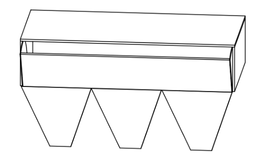
\includegraphics[width=0.6\columnwidth]{MainUnit.png}
  \caption{Main Control Module}
  \label{fig:main-control-module}
\end{figure}

An allowance of $0.180\text{ m}^3$ was adopted as the design target. The overall assembly of the main control module is shown in Figure \ref{fig:main-control-module}.
The central storage hopper is designed as a truncated rectangular pyramid (frustum) with a top face of $L = 1.0\text{ m} \times W = 0.5\text{ m}$ and a bottom opening of $a = b = 0.1\text{ m}$, consistent with the sliding-plate valve aperture. The slant height of the frustum walls is calculated from:
\begin{equation}
  h = \frac{(0.5\text{ m} - 0.1\text{ m})}{2} \times \tan(60^\circ) \approx 0.35\text{ m}
\end{equation}
The volume of each conical frustum section is given by the prismatoid formula, with corresponding dimensions illustrated in Figure \ref{fig:cone-dimensions}:
\begin{equation}
  V_{cone} = \frac{h}{3} (A_B + a_b + \sqrt{A_B \cdot a_b})
\end{equation}
where $A_B = 0.5\text{ m} \times 0.333\text{ m} = 0.165\text{ m}^2$ is the top-face area per section, and $a_b = 0.1\text{ m} \times 0.1\text{ m} = 0.01\text{ m}^2$ is the bottom-aperture area. Substituting into (3):
\begin{equation}
  V_{cone} \approx 0.02516\text{ m}^3 \times 3 \approx 0.075\text{ m}^3
\end{equation}

\begin{figure}[H]
  \centering
  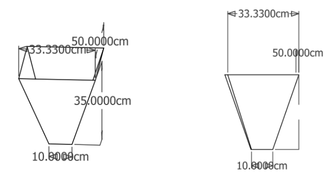
\includegraphics[width=0.8\columnwidth]{ConeDimensions.png}
  \caption{Cone Dimensions}
  \label{fig:cone-dimensions}
\end{figure}

\begin{figure}[H]
  \centering
  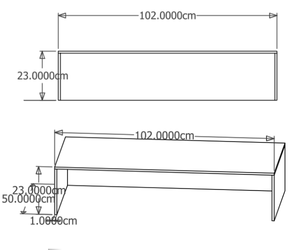
\includegraphics[width=0.8\columnwidth]{BoxDimensions.png}
  \caption{Box Dimensions}
  \label{fig:box-dimensions}
\end{figure}

The remaining volume is provided by a rectangular upper reservoir section of height $h_{rec}$, with the corresponding box dimensions shown in Figure \ref{fig:box-dimensions}. This is computed from:
\begin{equation}
  V_{rec} = V_{total} - V_{cones} = 0.180 - 0.075 = 0.105\text{ m}^3
\end{equation}
Solving for the rectangular section height with $L = 1.0\text{ m}$ and $W = 0.5\text{ m}$:
\begin{equation}
  h_{rec} = \frac{0.105\text{ m}^3}{1.0\text{ m} \times 0.5\text{ m}} = 0.21\text{ m}
\end{equation}

\begin{figure}[H]
  \centering
  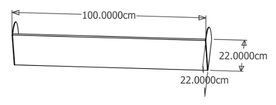
\includegraphics[width=0.8\columnwidth]{Hinged Hopper Lid.png}
  \caption{Hopper Lid Dimensions}
  \label{fig:hopper-lid-dimensions}
\end{figure}

The total hopper height is therefore $h_{cone} + h_{rec} = 0.35 + 0.21 = 0.56\text{ m}$, housed within an overall footprint of 102 cm $\times$ 50 cm at the top rim, as shown in Figure \ref{fig:hopper-lid-dimensions}. A separate funnel outlet is provided for each feeder node, directing feed into the trough.

\subsection{Dispensing Mechanism}

\begin{figure}[H]
  \centering
  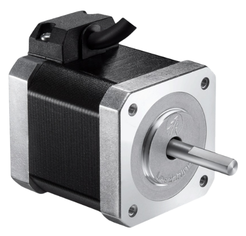
\includegraphics[width=0.5\columnwidth]{StepMotor.png}
  \caption{NEMA 17 Stepper Motor}
  \label{fig:stepper-motor}
\end{figure}

Feed release from the central hopper is controlled by a solenoid-actuated sliding plate valve (guillotine valve) positioned at the $0.1\text{ m} \times 0.1\text{ m}$ bottom aperture of the truncated pyramid. A 12 V DC push-pull solenoid drives the plate linearly, opening or closing the aperture under microcontroller command. This valve type was selected for its simplicity, low power consumption, and compatibility with granular feed materials that would jam rotary or butterfly valves.

An auger screw conveyor driven by a NEMA 17 stepper motor (shown in Figure \ref{fig:stepper-motor}) supplements the sliding valve for metered dispensing. By counting motor steps, the ESP32 can dispense feed in calibrated increments independently of gravity head pressure, improving dose accuracy across varying hopper fill levels. The hinged hopper lid is actuated by a secondary servo motor for automated refill access.

\subsection{Sensing Strategy and Component Selection}
Sensor selection was guided by the operating environment of a commercial piggery: high ambient humidity, a corrosive ammonia atmosphere, mechanical vibration from pig activity, and the need for low-cost scalability across multiple feeder nodes.

\begin{figure}[H]
  \centering
  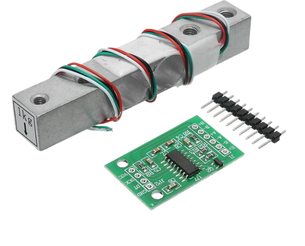
\includegraphics[width=0.5\columnwidth]{LoadCell.png}
  \caption{HX711 \& Straight Bar Load Cell}
  \label{fig:load-cell}
\end{figure}

\begin{itemize}
  \item \textbf{Feed Weight (Load Cell + HX711):} As shown in Figure \ref{fig:load-cell}, a strain-gauge load cell rated for the expected trough load is interfaced to an HX711 24-bit sigma-delta ADC. The HX711 communicates with the ESP32 over a dedicated two-wire serial interface, providing 10 or 80 samples per second. The trough weight is logged before and after each feeding event; the delta constitutes the dispensed mass. Consumption is derived by tracking weight loss between feeding cycles.

    \begin{figure}[H]
      \centering
      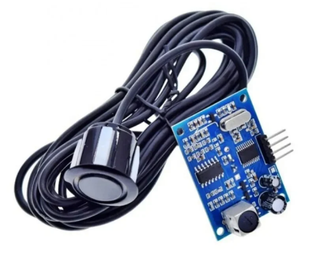
\includegraphics[width=0.7\columnwidth]{LevelSensor.png}
      \caption{JSN-SR04T Waterproof Ultrasonic Sensor}
      \label{fig:ultrasonic-sensor}
    \end{figure}

  \item \textbf{Water Availability (Level Sensor):} As depicted in Figure \ref{fig:ultrasonic-sensor}, a waterproof ultrasonic sensor is mounted above each pen's water trough. The ESP32 triggers an ultrasonic pulse and measures the echo time-of-flight to calculate the distance to the water surface. This determines the current water volume and triggers the solenoid valve to refill the trough when levels fall below the required baseline, ensuring constant water availability.

    \begin{figure}[H]
      \centering
      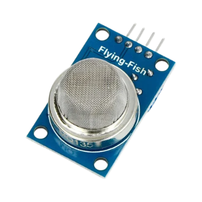
\includegraphics[width=0.5\columnwidth]{MQ-135.png}
      \caption{MQ-135 Air Quality Sensor}
      \label{fig:mq135-module}
    \end{figure}

  \item \textbf{Air Quality (MQ-135):} The MQ-135 electrochemical sensor, shown in Figure \ref{fig:mq135-module}, detects ammonia ($NH_3$), $CO_2$, and benzene vapors---the primary respiratory hazards in piggery environments arising from urine decomposition. The sensor's analog output is read by the ESP32's onboard ADC and compared against safe-range thresholds; exceedances trigger caretaker alerts on the dashboard.
\end{itemize}

\subsection{Wired Communication: RS-485 / MODBUS RTU}
The system specifies a hardwired network topology to eliminate dependence on wireless signal integrity in metal-framed piggery structures. RS-485 with the MODBUS RTU protocol was selected as the communication backbone for the following reasons:
\begin{itemize}
  \item Differential signaling on a twisted-pair bus provides high noise immunity in electrically harsh farm environments.
  \item The standard supports up to 32 nodes on a single bus segment at distances of up to 1,200 m, enabling future expansion of feeder modules without architectural redesign.
  \item MODBUS RTU is an industry-standard protocol with extensive ESP32 and Raspberry Pi library support, reducing firmware development overhead.
\end{itemize}
Each feeder-node ESP32 is interfaced to the bus via a MAX485 half-duplex transceiver IC. The Raspberry Pi master polls each slave node at configurable intervals, retrieves sensor data packets, and writes dispensing commands. A unique MODBUS device address is assigned to each feeder module during commissioning.

\subsection{Application Layer and Data Persistence}
The centralized user interface (UI) is hosted on the Raspberry Pi and rendered through a 7-inch DSI touchscreen mounted on the main control module enclosure. The software stack utilizes a lightweight web-based architecture to ensure low-latency updates:
\begin{itemize}
  \item \textbf{Backend Stack:} A Flask-based web server manages the API endpoints for the dashboard. It interfaces with an SQLite database for ACID-compliant persistence of timestamped consumption logs, feeding schedules, and air-quality telemetry.
  \item \textbf{Frontend Stack:} A Chromium kiosk browser displays a dashboard built with responsive numeric gauges and time-series charts for real-time monitoring and historical trend visualization. It includes configuration panels for feeding schedules and alert logs for threshold exceedances.
  \item \textbf{Fault Tolerance:} All data is stored locally, ensuring continuous operation during internet outages, which is a primary concern identified in the study's scope and limitations. To address potential grid instability, a UPS module with 18650 lithium cells provides bridge power, ensuring that the SQLite database maintains integrity during short-duration power interruptions.
  \item \textbf{LoRa-SMS Alert Gateway:} A background Python thread runs alongside the Flask backend. It continuously monitors the SQLite database for newly generated threshold exceedances. To optimize radio duty cycles and prevent packet collisions, the gateway implements a message-queuing protocol, bundling non-critical alerts and transmitting them via the LoRa link to the remote LoRa-GSM gateway at configured intervals or triggering immediate LoRa transmission for critical air-quality hazards. The remote gateway then forwards each alert as an SMS to the caretaker's mobile phone.
\end{itemize}

\subsection{Consumption Baseline and Anomaly Detection}
A pig's health status is closely linked to its feeding and drinking behavior; measurable deviations in dietary intake are often among the first observable indicators of illness \cite{dingcong2017monitoring,sadeghi2023improving}. The system establishes per-module baselines using a rolling time-window approach consistent with data-driven livestock monitoring methods reported in the literature \cite{racewicz2021welfare,sadeghi2023improving}. Let $C_i$ denote the feed consumed in session $i$. The rolling mean over a window of $N$ sessions is:
\begin{equation}
  \mu_N = \frac{1}{N} \sum_{i=t-N+1}^{t} C_i
\end{equation}
A deviation alert is generated when the current session's consumption $C_t$ falls outside the band $[\mu_N - k\sigma, \mu_N + k\sigma]$, where $\sigma$ is the rolling standard deviation and $k$ is a configurable sensitivity coefficient (default $k=2$). This statistical approach reduces false positives arising from natural day-to-day variation while reliably flagging behaviorally significant declines \cite{sadeghi2023improving,racewicz2021welfare}.

\subsection{Evaluation Metrics and Verification Protocol}
System performance will be assessed against quantitative metrics aligned with the project's specific objectives. These metrics are intended to reflect the reliability of dispensing, sensing, communication, and health-monitoring functions commonly emphasized in precision livestock and embedded monitoring studies \cite{adeoye2025animalia,beyondtech2025smart,sadeghi2023improving}. To ensure system reliability and accuracy prior to full-scale deployment, a rigorous testing protocol will be executed to systematically validate these metrics.

\textbf{Quantitative Metrics:}
\begin{itemize}
  \item \textbf{Feed Dispensing Accuracy (FDA):} Percentage agreement between the target dispensed mass and the gravimetrically measured actual dispensed mass across a calibration trial of 30 dispensing events per module. A minimum passing threshold of $\geq 95\%$ is required for the system to be considered operationally accurate \cite{adeoye2025animalia,dingcong2017monitoring}:
    \begin{equation}
      FDA = \left(1 - \frac{|M_{target} - M_{actual}|}{M_{target}}\right) \times 100\%
    \end{equation}
  \item \textbf{Alert Response Accuracy (ARA):} Proportion of simulated consumption anomaly events correctly detected and flagged by the baseline algorithm within one polling cycle. A minimum passing threshold of $\geq 90\%$ is required to validate the reliability of the anomaly detection logic \cite{sadeghi2023improving,racewicz2021welfare}:
    \begin{equation}
      ARA = \frac{\text{True Positive Alerts}}{\text{Total Induced Events}} \times 100\%
    \end{equation}
  \item \textbf{System Uptime ($U_{sys}$):} Measured over a 72-hour continuous operation trial, consistent with endurance validation practices for embedded monitoring systems \cite{beyondtech2025smart,adeoye2025animalia}:
    \begin{equation}
      U_{sys} = \frac{T_{total} - T_{downtime}}{T_{total}} \times 100\%
    \end{equation}
    where $T_{total}$ is the total trial duration in hours and $T_{downtime}$ is the cumulative time during which sensor polling or the dashboard was unavailable.
  \item \textbf{Data Display Latency:} Time elapsed between a sensor reading being acquired at the feeder node and its appearance on the dashboard, measured across 50 consecutive poll cycles. Target threshold: $\le 2$ seconds \cite{beyondtech2025smart,adeoye2025animalia}.
  \item \textbf{SMS Delivery Rate (SDR):} The end-to-end percentage of alert messages successfully delivered as SMS to the caretaker's mobile phone via the LoRa-GSM gateway, compared to the total number of alerts generated by the central unit. A minimum passing threshold of $\geq 95\%$ is required to confirm reliable remote notification delivery \cite{beyondtech2025smart,reza2025review}:
    \begin{equation}
      SDR = \frac{\text{Total SMS Delivered}}{\text{Total Alerts Generated}} \times 100\%
    \end{equation}
  \item \textbf{End-to-End Alert Latency:} The time elapsed between an alert being generated by the Analytical Engine and the corresponding SMS being successfully delivered to the caretaker's mobile phone, encompassing LoRa transmission, gateway processing, and GSM delivery. Target threshold: $\le 30$ seconds per alert message \cite{beyondtech2025smart,reza2025review}.
\end{itemize}

\subsection{Verification Phases}
The testing protocol is divided into three primary phases to validate both the hardware edge nodes and the central software orchestration. This phased approach is consistent with common validation practice in embedded sensing, livestock-monitoring, and agricultural automation studies, where component calibration, communication validation, and full-system integration are assessed separately before deployment \cite{adeoye2025animalia,dingcong2017monitoring,beyondtech2025smart}:
\begin{itemize}
  \item \textbf{Phase 1: Sensor Calibration and Hardware Validation}
    \begin{itemize}
      \item \textbf{Gravimetric Testing (FDA Validation):} The load cell and HX711 assemblies will be calibrated using standard reference weights across a range of 0 to 5 kg, covering the expected trough load. A minimum of 10 calibration trials per load cell will be conducted. Linearity and hysteresis will be evaluated across the expected load range to ensure Feed Dispensing Accuracy meets the $\geq 95\%$ passing threshold \cite{dingcong2017monitoring,adeoye2025animalia}.
      \item \textbf{Water Level Calibration:} The ultrasonic level sensors will be validated against manual depth measurements using a calibrated dipstick across a range of operational trough depths. A minimum of 10 trials per sensor will be conducted to establish a precise time-of-flight to depth conversion factor and verify the threshold-trigger logic for the solenoid valves \cite{adeoye2025animalia,beyondtech2025smart}.
      \item \textbf{Environmental Baseline:} The MQ-135 sensors will undergo a minimum 48-hour burn-in period followed by calibration in a controlled, clean-air environment to establish a baseline resistance ($R_0$) before exposure to the piggery atmosphere. Sensors will then be tested against known ammonia concentrations in the range of 10 to 300 ppm to verify threshold response accuracy prior to deployment \cite{sadeghi2023improving,adeoye2025animalia,yamsakul2025machine}.
    \end{itemize}
  \item \textbf{Phase 2: Communication and Firmware Testing}
    The RS-485 wired bus will undergo signal integrity testing with all feeder nodes active on the bus simultaneously. A digital storage oscilloscope will be used to verify that differential voltage levels meet the RS-485 standard minimum of $\pm 1.5$ V and ensure adequate common-mode noise rejection. MODBUS RTU packet loss rates will be quantified under simulated electrical noise conditions at the maximum prototype cable length. A packet loss rate of $\leq 1\%$ is required to confirm robust master-slave polling before proceeding to system integration \cite{beyondtech2025smart,adeoye2025animalia}.
  \item \textbf{Phase 3: System-Level Integration (Uptime, Latency, ARA, and LoRa-SMS Validation)}
    A 72-hour continuous operation trial will be conducted in a controlled environment to measure System Uptime ($U_{sys}$) and verify that Data Display Latency remains $\le 2$ seconds. To validate the rolling-window anomaly detection, simulated consumption drops will be manually injected into the data stream to test the Alert Response Accuracy (ARA) of the Python backend. Furthermore, the LoRa-to-SMS notification pipeline will undergo end-to-end testing. Simulated consumption drops will be injected to trigger alerts, and the SMS Delivery Rate (SDR) and End-to-End Alert Latency will be measured at varying distances between the main control module and the LoRa-GSM gateway to validate the reliability of remote caretaker notifications \cite{dingcong2017monitoring,sadeghi2023improving,reza2025review}.
\end{itemize}

\subsection{Deployment Plan}
The transition from the laboratory prototype to field operation in a commercial piggery will follow a structured, four-phase deployment strategy to minimize disruption to existing farm operations:
\begin{itemize}
  \item \textbf{Phase 1: Site Assessment and Electrical Routing:} An evaluation of the piggery's physical layout will determine the optimal routing for the RS-485 twisted-pair cables and DC power distribution. Cable trajectories will be explicitly planned to avoid electromagnetic interference (EMI) from existing high-voltage farm equipment or large motors. This phase must produce three deliverables before installation proceeds: a cable routing diagram, a DC power distribution plan, and an EMI risk assessment identifying high-interference zones within the facility.
  \item \textbf{Phase 2: Physical Installation:} The central $0.18\text{ m}^3$ hopper, auger mechanism, and main control module (Raspberry Pi) will be securely mounted at the centralized feeding station. Individual feeder nodes (ESP32 enclosures, load cells, and level sensors) will be mechanically integrated into the pen structures. The level sensors will be securely mounted directly above the water troughs, and the plumbing will be retrofitted to integrate the automated solenoid valves. Installation is considered complete only after all nodes pass a hardware checklist confirming that all units are powered, all sensors are returning non-zero readings, and all MODBUS device addresses have been successfully assigned and acknowledged by the master.
  \item \textbf{Phase 3: Commissioning and Baseline Initialization:} Once powered, unique MODBUS device addresses will be assigned to each feeder node. The system will initially operate in a "silent monitoring" phase (e.g., 7 to 14 days). During this period, the system will dispense feed and log data to the SQLite database without triggering health alerts, allowing the rolling-window algorithm to establish accurate, pen-specific consumption baselines ($\mu_N$). Anomaly detection will not be activated until a minimum of $N = 14$ feeding sessions have been recorded per module, ensuring the rolling-window baseline is statistically sufficient before alerts are generated.
  \item \textbf{Phase 4: Caretaker Turnover and Training:} Farm operators will undergo practical training on utilizing the Raspberry Pi touchscreen interface. This includes instructing them on how to interpret the time-series charts, modify feeding schedules, address alert logs, and perform routine maintenance such as clearing auger jams or cleaning the optical/gas sensor interfaces. Turnover is considered complete only when each caretaker can independently demonstrate three competencies without assistance: interpreting and responding to a generated alert, modifying a feeding schedule on the dashboard, and performing basic sensor maintenance.
\end{itemize}
